%!TEX TS-program = xelatex
\documentclass[]{friggeri-cv}
\usepackage{afterpage}
\usepackage{hyperref}
\usepackage{color}
\usepackage{xcolor}
\usepackage{float}
\hypersetup{
    pdftitle={},
    pdfauthor={},
    pdfsubject={},
    pdfkeywords={},
    colorlinks=false,       
   allbordercolors=white   
}
\addbibresource{bibliography.bib}
\RequirePackage{xcolor}
\definecolor{pblue}{HTML}{0395DE}

\begin{document}
\header{Saïd}{Ziani}
      {Développeur informatique}
      
\fcolorbox{white}{gray}{\parbox{\dimexpr\textwidth-2\fboxsep-2\fboxrule}{%
.....
}}

\begin{aside}
  \section{Adresse}
    05 Chemin Ahmed Boumazouza,
    El-madania, Alger, Algérie
    ~
    ~
  \section{Tel \& Linkedin}
    +213797668521
    \href{https://www.linkedin.com/in/sa%C3%AFd-ziani-008487120/}{\textbf{Saïd Ziani}}
    ~
    ~
  \section{Mail}
    \href{mailto:saidziani.pro@gmail.com}{\textbf{saidziani.pro@}\\gmail.com}
    ~
    ~
  \section{Web \& Git}
    \href{http://www.openmindsclub.net}{openmindsclub.net}
    \href{http://www.openmindsclub.net/ip8}{installparty.net}
    \href{https://github.com/saidziani}{github.com/saidziani}
    ~
    ~
  \section{Programmation}
    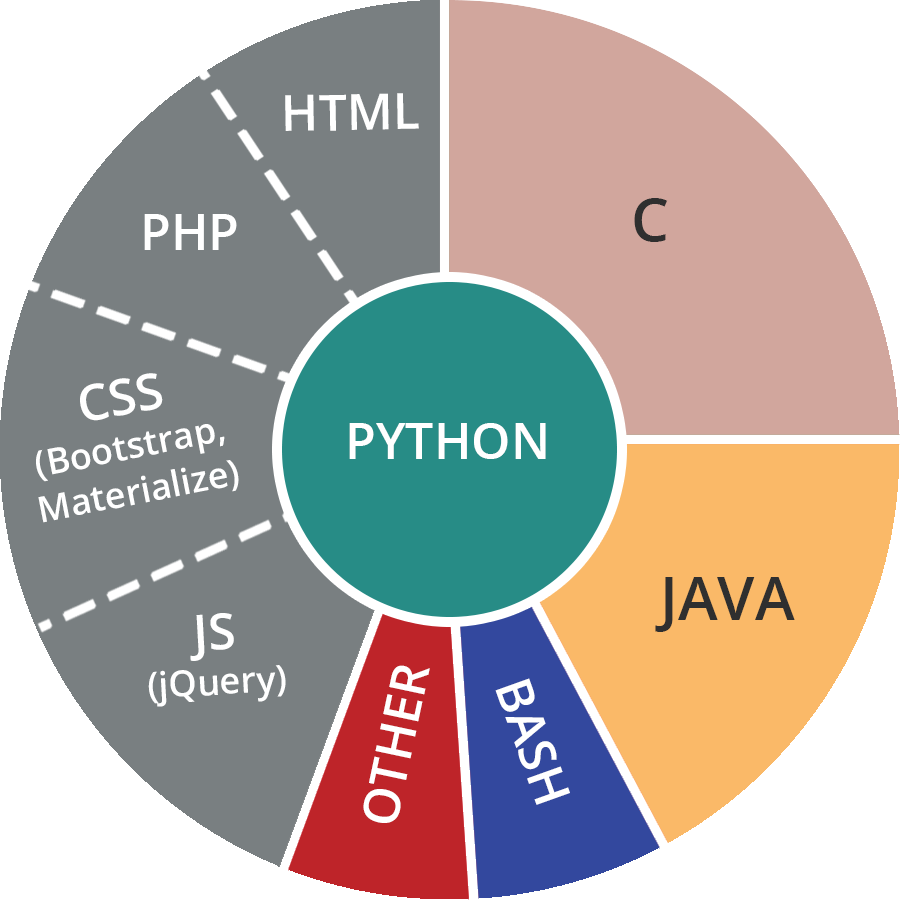
\includegraphics[scale=0.1]{img/programmation.png}
    ~
    ~
  \section{OS Préférence}
    \textbf{GNU/Linux}
\includegraphics[scale=0.40]{img/5stars.png}
    \textbf{Unix}
\includegraphics[scale=0.40]{img/4stars.png}
    \textbf{MacOS}
\includegraphics[scale=0.40]{img/2stars.png}
    \textbf{Windows}
\includegraphics[scale=0.40]{img/1stars.png}
    ~
    ~
  \section{Bureautique}
    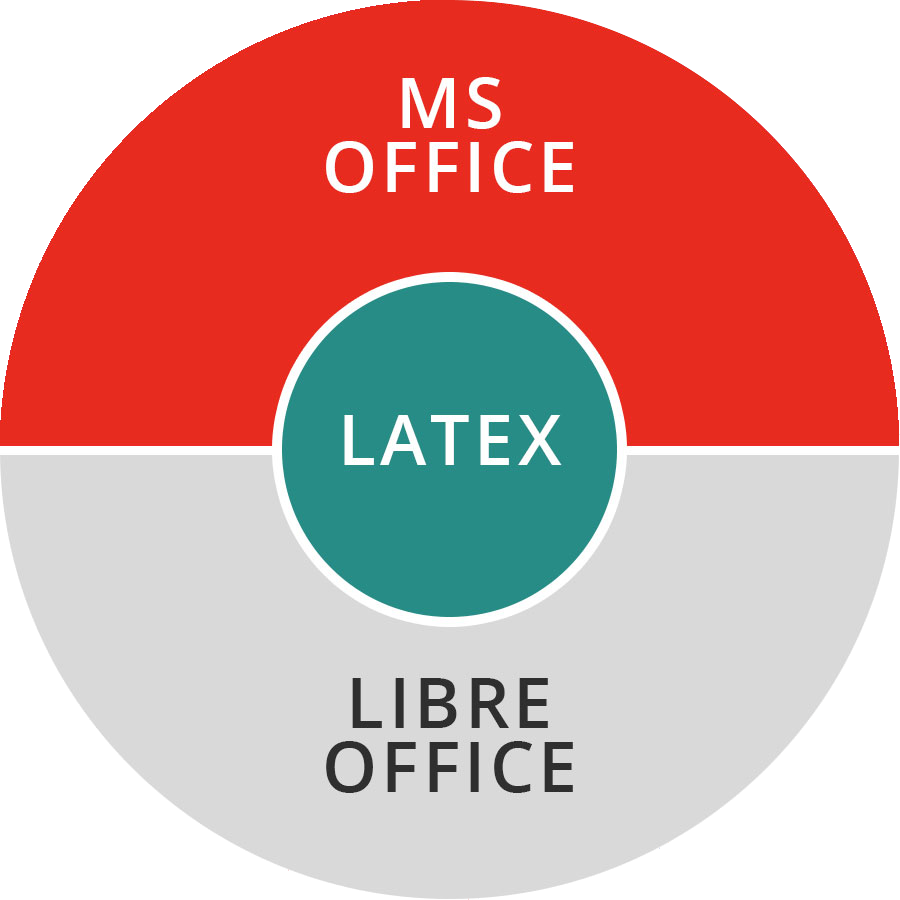
\includegraphics[scale=0.1]{img/bureautique.png}
    ~
\end{aside}
\vspace{0.42cm}
\section{Expérience}
\begin{entrylist}
  \entry
    {Depuis 06/17}
    {Développeur PHP}
    {\href{http://www.hivedigit.com/}{HiveDigit}, Alger}
    {B2B, E-commerce, Yii framework, PHP, Plateform, entre professionnelles, backend et frontend, mise à jour, entretien et maintenace (bugs, securité..)\\}
  \entry
    {Depuis 09/16}
    {Développeur}
    {Club Open Minds, USTHB, Alger}
    {Développement de plusieurs solutions informatiques, principalement des sites web et des applications de gestion,\\veille et administration des bases de données(Mysql).\\}
  \entry
    {Depuis 01/16}
    {Développeur Freelance}
    {}
    {Création de plusieurs sites web, principalement des sites vitrines et des portfolios souvent accompagné d'une administration dynamique.\\
    Exemple:Portfolio d'un graphiste/photographe \href{http://www.samirouferhat.com/}{\textbf{clicker ici}}.\\}
  \entry
    {09/15 - 06/16}
    {Concepteur et développeur}
    {COSIDER CANALISATIONS, Alger}
    {Conception, développement et intégration d'un module d'ERP destiné à la gestion des approvisionnements, dans le cadre de mon projet de fin d'étude de Licence.\\}
  \entry
    {06/15 - 08/15}
    {Concepteur système d'information}
    {COSIDER CANALISATIONS, Alger}
    {Mise en place d'un système d'information traitant les différentes procédures du fonctionnement de la direction des approvisionnements et de la sous-traitance.\\}
\end{entrylist}
\vspace{1cm}
\section{Enseignement}
\begin{entrylist}
  \entry
    {Depuis 09/16}
    {Master en  Système informatique intelligent}
    {USTHB, Alger}
    {Apprentissage automatique(Machine learning), représentation des connaissances et formalisation du raisonnement, Réseaux de neurones, E-commerce et webservices, Base de données avancée(Oracle) et sécurité informatique\\}
  \entry
    {09/13 - 06/16}
    {Licence en informatique général- Mention: Très bien}
    {USTHB, Alger}
    {Mathématique et physique, Recherche opérationnelle, Programmation et développement web,  Base de données(Oracle) et électronique analogique.\\}
  \entry
    {06/12}
    {BAC Science- Mention: Bien}
    {Lycée Mohamed Bodiaf, El-madania, Alger}
    {Mathématique, Physique, Science, Philosophie et langues.}
\end{entrylist}

\newpage
\section{Activités}
\begin{entrylist}
  \entry
    {depuis 05/16}
    {CTF- Capture The Flag}
    {}
    {Étant un passionné de la sécurité des systèmes informatiques, j'ai intégré l'équipe \href{https://web.facebook.com/F0xHo2Nd/}{\textbf{Fox-Hound}}, depuis je participe régulièrement aux compétitions de CTF (challenges de sécurité permettant de s’entraîner aux attaques fictives d’intrusion) ce qui m'a permis d'élargir mes compétences pratiques le tout dans un esprit plaisant et collaboratif.\\}
  \entry
    {03/17}
    {Hack!t}
    {}
    {Participant émérite du Hackaton organisé par l'ESI, notre projet portant sur la gestion intelligente d'un cabinet médical, nous hissa à la troisième place du classement final.\\}
  \entry
    {12/16}
    {Algeria Web Awards}
    {}
    {Finaliste des AWA catégorie "Association" avec le site \href{http://www.openmindsclub.net/}{\textbf{openmindsclub.net}}, je fus développeur du site et présentateur du projet.\\
    (AWA: l’événement qui réunit tout les acteurs de la scène web algérienne).\\}
    
\end{entrylist}

\begin{aside}
~
~
~
  \section{Langues}
    \textbf{Arabe}
\includegraphics[scale=0.40]{img/5stars.png}
    \textbf{Français}
\includegraphics[scale=0.40]{img/5stars.png}
    \textbf{English}
\includegraphics[scale=0.40]{img/3stars.png}
    ~
    ~
    ~
  \section{Compétences personnelles}
    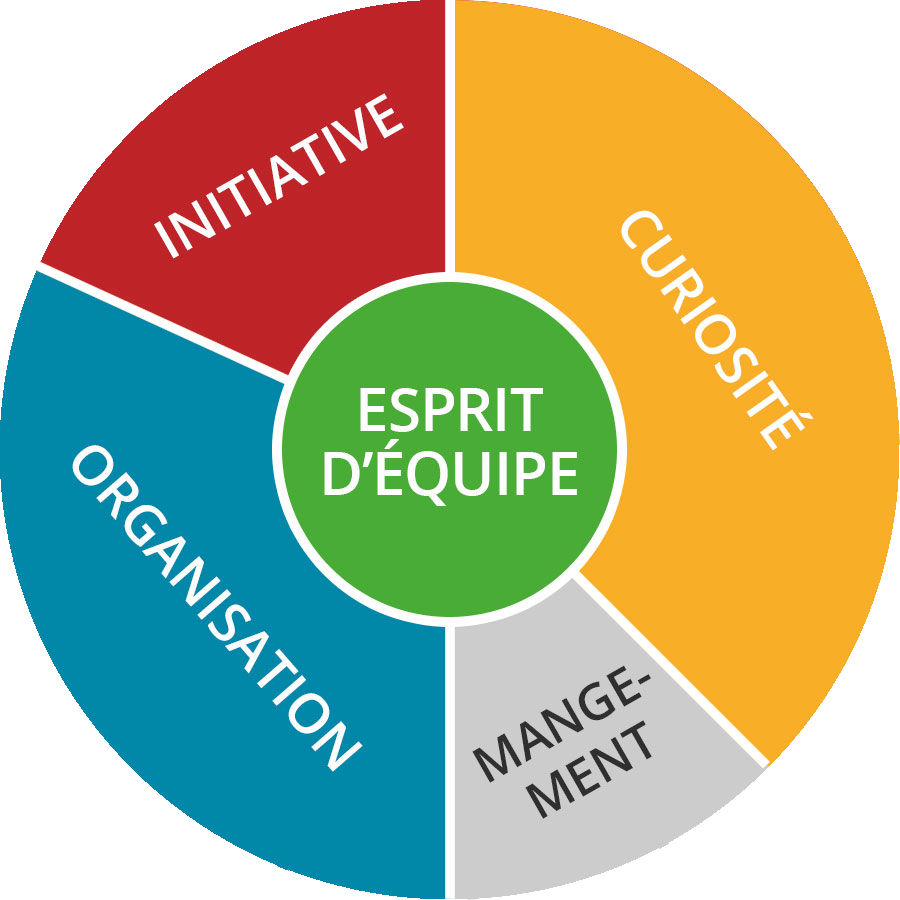
\includegraphics[scale=0.1]{img/personnel.png}
    ~
\end{aside}

\section{Autres}
\begin{entrylist}
  \entry
    { }
    {Activités sportifs}
    {Handball et natation}
    {Depuis l'âge de 6 ans, j'ai choisis le Handball comme sport préféré, j'ai joué dans plusieurs équipes, je me suis déplacé à plusieurs reprise dans différents club, en parallèle j'étais nageur dans un club de natation à Alger.\\}
  \entry
    {}
    {Job d'été}
    {}
    {Je consacre chaque été une partie de mon temps à des mini job,j'ai travaillé comme préparateur/serveur dans un salon de glace quatre été de suite, cela m'a permis de côtoyer le monde du travail mais aussi d’acquérir une certaine tolérance et compréhension envers les clients.}
  \entry
    { }
    {Open Minds Club}
    {\href{http://www.openmindsclub.net}{openmindsclub.net}}
    {La plus belle expérience, et de loin, est celle de mon adhésion au club scientifique Open Minds,ça m'a données la chance de montré le peu de savoir que j'avais et de développer ce dernier.\\}
\end{entrylist}

\end{document}
